% ============================================================
% Lecture 1 -- Basic Statistics and Introduction to R
% ============================================================
\section{Basic Statistics and Introduction to R}\label{sec:L01}

\lectureheader{1}{z1RfnVy8Oak}{Week-1 slides \texttt{Jan26notes.pdf} (with the instructor's handwritten annotations)}

\begin{guiding*}
By the end of this lecture you should be able to:
\begin{itemize}
  \item say what R is, where it came from, and how to install R and RStudio (and what the Python equivalents are);
  \item classify data as categorical, discrete numeric or continuous numeric;
  \item describe numerical data by its \emph{centre}, \emph{spread} and \emph{shape}, and compute the mean, median, mode, variance, standard deviation and inter-quartile range;
  \item load a built-in data frame, look at it with \texttt{head}, \texttt{tail} and indexing, and make the five-number summary, histogram and scatter plots.
\end{itemize}
\end{guiding*}

\subsection{Motivation}
The course is about \emph{linear statistical models}, but every model starts with data.
Before we write down $Y = X\beta+\eps$ we have to know how to read a data set, summarise it,
and draw pictures of it. The first week therefore reviews basic descriptive statistics and
introduces the computing environment. The instructor's slides open with a light-hearted
``statutory warning'': he tends to speak quickly, and students should ask him to repeat anything
that is unclear. The same advice applies to these notes: work through every example yourself,
in the companion notebook if you like.

\subsection{The R environment}
The slides describe R as follows.
\begin{itemize}
  \item R is an open-source programming language for statistical computing. It runs on Linux, Windows and Mac~OS, and it is free. The project web page is \url{http://www.r-project.org}.
  \item R is modelled on the languages S and S-Plus. S was developed in the late 1980s at AT\&T Bell Labs.
  \item The R project was started in 1995 by Robert Gentleman and Ross Ihaka of the Statistics Department of the University of Auckland (\emph{Journal of Computational and Graphical Statistics} 5:3, 299--314, 1996). It is now maintained by the R core development team with many contributors.
  \item R is downloaded from \url{https://cloud.r-project.org}. RStudio is an \vocab{integrated development environment} (IDE) for R.
\end{itemize}
There is plenty of help available on the web, for example the R-bloggers site.

\begin{note}[Supplementary: the Python counterpart used in this book]
Throughout these notes the R demonstrations are translated into Python. The ingredients are
\texttt{numpy} (arrays and linear algebra), \texttt{pandas} (data frames),
\texttt{matplotlib}/\texttt{seaborn} (graphics), \texttt{scipy.stats} (distributions) and
\texttt{statsmodels} (linear models). The IDE is VS~Code with the Jupyter extension. Setup
instructions are in the \texttt{README.md} at the root of the project.
\end{note}

\subsection{Kinds of data}
\begin{definition}[Types of data]\label{def:L01-datatypes}
The slides distinguish three kinds of data.
\begin{enumerate}
  \item \vocab{Categorical data}: each observation belongs to one of a set of labels, for example $\{0,1\}$ or $\{A,B,\dots\}$.
  \item \vocab{Discrete numeric data}: numbers that naturally take only discrete values, for example counts.
  \item \vocab{Continuous numeric data}: numbers that can take any value in an interval, for example temperature or a stock price.
\end{enumerate}
\end{definition}
The slides refer to S.\,S.~Stevens, ``On the theory of scales of measurement'',
\emph{Science} 103 (1946), 677--680, for a finer classification of measurement data. As typical
examples of numeric data the slides mention daily temperatures and the earnings of a stock in a
stock market. Such data are visualised with histograms and boxplots.

\begin{note}[Supplementary: Stevens' scales]
Stevens' paper is best known for its four scales of measurement: \emph{nominal} (labels only),
\emph{ordinal} (labels with an order), \emph{interval} (differences are meaningful, zero is
arbitrary, e.g.\ temperature in $^\circ$F) and \emph{ratio} (a true zero, e.g.\ length). The
scale determines which summaries make sense. A mean of nominal codes is meaningless, and a
ratio of two Fahrenheit temperatures has no physical meaning.
\end{note}

\subsection{Centre, spread and shape}
For numerical data the slides single out three key features. We make each one precise. Let
$x_1,\dots,x_n$ be the data and $x_{(1)}\le\dots\le x_{(n)}$ the ordered data.

\begin{definition}[Measures of centre]\label{def:L01-centre}
\begin{itemize}
  \item The \vocab{mean} (average) is $\bar x = \frac1n\sum_{i=1}^n x_i$. If the distinct values $x_1,\dots,x_k$ occur with frequencies $f_1,\dots,f_k$ ($\sum f_i=n$), then $\bar x = \frac1n\sum_{i=1}^k f_ix_i$. This frequency form is written on the slide.
  \item The \vocab{median} is the middle ordered value: $x_{((n+1)/2)}$ if $n$ is odd, and $\tfrac12\paren{x_{(n/2)}+x_{(n/2+1)}}$ if $n$ is even.
  \item The \vocab{mode} is the most frequently occurring value.
\end{itemize}
\end{definition}

\begin{definition}[Measures of spread]\label{def:L01-spread}
\begin{itemize}
  \item The (sample) \vocab{variance} is $s^2=\frac{1}{n-1}\sum_{i=1}^n (x_i-\bar x)^2$. This is R's \texttt{var}. The \vocab{standard deviation} is $s=\sqrt{s^2}$ (R's \texttt{sd}).
  \item The \vocab{inter-quartile range} is $\mathrm{IQR}=Q_3-Q_1$, where $Q_1$ and $Q_3$ are the first and third quartiles (the $25\%$ and $75\%$ quantiles).
\end{itemize}
\end{definition}

The \emph{shape} of the data describes, for example, whether it is symmetric or skewed about its
centre, and which values are more likely than others. The instructor's sketch shows a
symmetric histogram around $0$ and an asymmetric one with a long tail. Next to the sketch he
writes that most of the data lie in an ``essential range'' from mean$-3\,$SD to mean$+3\,$SD.
The next result makes this precise for \emph{every} data set.

\begin{proposition}[Supplementary: Chebyshev's inequality for data]\label{prop:L01-cheb}
Let $\sigma_n^2=\frac1n\sum (x_i-\bar x)^2$ and suppose $\sigma_n>0$. For every $k>0$, the proportion of data points with
$\abs{x_i-\bar x}\ge k\sigma_n$ is at most $1/k^2$. In particular at least $8/9\approx 89\%$ of any
data set lies within $3\sigma_n$ of the mean.
\end{proposition}
\begin{proof}
Let $A=\{i:\abs{x_i-\bar x}\ge k\sigma_n\}$ and let $\# A$ be its size. Every term in the sum below
is non-negative, and for $i\in A$ we have $(x_i-\bar x)^2\ge k^2\sigma_n^2$. Therefore
\[
n\sigma_n^2=\sum_{i=1}^n (x_i-\bar x)^2 \;\ge\; \sum_{i\in A}(x_i-\bar x)^2\;\ge\; \#A\cdot k^2\sigma_n^2 .
\]
Dividing by $nk^2\sigma_n^2>0$ gives $\#A/n\le 1/k^2$. Taking $k=3$ gives the second statement.
\end{proof}

For roughly bell-shaped data the proportion inside mean $\pm 3\,$SD is much higher, about
$99.7\%$. That is why the instructor calls it the essential range.

\begin{proposition}[Supplementary: the mean and the median as best constants]\label{prop:L01-bestconst}
For data $x_1,\dots,x_n$,
\begin{enumerate}
  \item $c\mapsto\sum_{i=1}^n (x_i-c)^2$ is minimised uniquely at $c=\bar x$;
  \item $c\mapsto\sum_{i=1}^n \abs{x_i-c}$ is minimised at any median.
\end{enumerate}
\end{proposition}
\begin{proof}
(1) Write $x_i-c=(x_i-\bar x)+(\bar x-c)$ and expand:
\[
\sum_{i}(x_i-c)^2=\sum_i (x_i-\bar x)^2 + 2(\bar x-c)\sum_i (x_i-\bar x) + n(\bar x-c)^2 .
\]
The middle sum is $\sum_i x_i - n\bar x=0$. So $\sum(x_i-c)^2=\sum(x_i-\bar x)^2+n(\bar x-c)^2$,
which is smallest exactly when $c=\bar x$.

(2) Let $g(c)=\sum_i\abs{x_i-c}$. The function $g$ is convex and piecewise linear. At a point $c$
that is not a data value its derivative is $\#\{i:x_i<c\}-\#\{i:x_i>c\}$. This is negative while
fewer than half of the points lie below $c$ and positive once more than half do. A convex
function is minimised where its slope changes sign, which is at a median.
\end{proof}
The first identity, ``total squared deviation $=$ deviation about the mean $+$ $n\times$(distance
of the mean)$^2$'', is the simplest case of the Pythagorean decompositions behind all of least
squares. We will meet it again in \cref{sec:L08,sec:L12}.

\begin{example}[Summaries by hand]\label{ex:L01-summary}
Consider the nine observations $3,7,8,5,12,14,21,13,18$.
\end{example}
\noindent\emph{Solution.} Ordered: $3,5,7,8,12,13,14,18,21$.
\begin{itemize}
  \item Mean: $\sum x_i=101$, so $\bar x=101/9=11.2222$.
  \item Median: $n=9$ is odd, so the median is $x_{(5)}=12$.
  \item Variance: $\sum x_i^2 = 9+25+49+64+144+169+196+324+441=1421$. Hence
  $\sum (x_i-\bar x)^2=\sum x_i^2-n\bar x^2 = 1421-101^2/9 = 1421-1133.4444=287.5556$, and
  $s^2=287.5556/8=35.9444$, $s=5.9954$.
  \item Quartiles: R's default rule (\texttt{type = 7}, also NumPy's default) puts the $q$-quantile at
  ordered position $1+(n-1)q$. For $q=0.25$ this is position $3$, so $Q_1=x_{(3)}=7$. For $q=0.75$ it is
  position $7$, so $Q_3=x_{(7)}=14$. Hence $\mathrm{IQR}=7$.
  \item The five-number summary is $(\min,Q_1,\text{median},Q_3,\max)=(3,7,12,14,21)$ and the mean is $11.22$.
  The mean is below the median here: the lower tail ($3,5$) pulls it down more than the upper tail pushes it up.
\end{itemize}
These numbers are reproduced in the notebook \nb{week01/L01\_basic\_stats\_intro.ipynb}.

\subsection{Data sets and data frames}
R ships with many data sets. The command \texttt{data()} lists the installed ones, and the
instructor strongly encourages students to pick a data set and repeat the class experiments on it.

\begin{definition}[Data frame]\label{def:L01-dataframe}
A \vocab{data frame} is a rectangular collection of \emph{variables} (the columns) and
\emph{observations} (the rows).
\end{definition}

\begin{example}[The \texttt{airquality} data]\label{ex:L01-airquality}
\texttt{?airquality} describes daily air-quality measurements in New York (May--September 1973).
It is a data frame with $153$ rows and $6$ columns: \texttt{Ozone}, \texttt{Solar.R}, \texttt{Wind},
\texttt{Temp}, \texttt{Month} and \texttt{Day}. The slides use it to show the following commands.
\begin{itemize}
  \item \texttt{head(airquality)} and \texttt{tail(airquality)} show the first and the last six rows; with \texttt{n = 10}, \texttt{head} shows ten rows.
  \item \texttt{airquality[148,4]} returns \texttt{63}, the entry in row 148 and column 4 (\texttt{Temp}). The same value is \texttt{airquality\$Temp[148]}.
  \item \texttt{airquality[148,]} is the whole 148th row. \texttt{airquality[,c(1,4)]} gives the \texttt{Ozone} and \texttt{Temp} columns for all rows; \texttt{c()} builds the vector of column numbers.
  \item \texttt{summary(airquality\$Temp)} prints the five-number summary together with the mean:
  \[
  \text{Min }56,\quad Q_1\ 72,\quad \text{Median }79,\quad \text{Mean }77.88,\quad Q_3\ 85,\quad \text{Max }97.
  \]
\end{itemize}
\end{example}

\begin{note}[Indexing pitfall]
R counts from $1$, Python from $0$. In pandas, R's \texttt{airquality[148,4]} is
\texttt{aq.iloc[147, 3]} or \texttt{aq.loc[147, "Temp"]}. The value is again $63$.
\end{note}

\subsection{First plots}
The slides then make three kinds of plot.
\begin{itemize}
  \item \texttt{hist(airquality\$Temp)}: a histogram. Temperatures range from $56$ to $97$ with a peak in the high $70$s and low $80$s, and the histogram is mildly left-skewed.
  \item \texttt{plot(airquality\$Temp)}: the values plotted against their index. Because the rows are in date order, this is a time plot. It shows temperatures rising into the summer and falling in September.
  \item \texttt{plot(airquality\$Ozone, airquality\$Temp)}: a scatter plot. Days with higher ozone tend to be hotter.
  \item \texttt{plot(airquality)}: a matrix of scatter plots of every pair of variables.
\end{itemize}

\begin{figure}[ht]
\centering
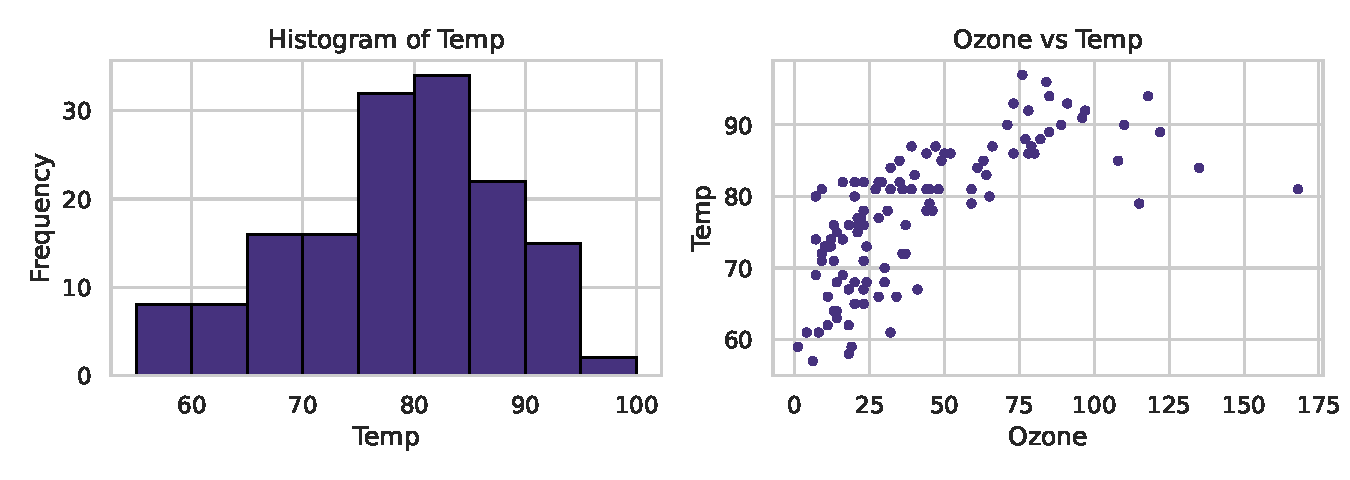
\includegraphics[width=0.95\textwidth]{figures/L01_airquality.pdf}
\caption{Histogram of \texttt{Temp} and scatter plot of \texttt{Temp} against \texttt{Ozone} (\texttt{airquality}).}
\label{fig:L01-airquality}
\end{figure}

\subsection{External packages}
R can be extended with packages. \texttt{install.packages("UsingR")} installs the package
\texttt{UsingR}, which contains many data sets, and \texttt{library("UsingR")} adds it to the
current workspace. Likewise \texttt{install.packages("tidyverse")} and
\texttt{library("tidyverse")} load \texttt{ggplot2}, the graphics system used in
\cref{sec:L02,sec:L03}.

\subsection{Computation}
The R commands of this lecture translate to Python as follows.
\begin{center}
\begin{tabular}{@{}ll@{}}\hline
R & Python (pandas / matplotlib)\\\hline
\texttt{head(airquality, n=10)} & \texttt{aq.head(10)}\\
\texttt{airquality[148,4]} & \texttt{aq.iloc[147, 3]}\\
\texttt{airquality[,c(1,4)]} & \texttt{aq.iloc[:, [0, 3]]}\\
\texttt{summary(airquality\$Temp)} & \texttt{aq.Temp.describe()}\\
\texttt{hist(airquality\$Temp)} & \texttt{plt.hist(aq.Temp)}\\
\texttt{plot(airquality)} & \texttt{pd.plotting.scatter\_matrix(aq)}\\\hline
\end{tabular}
\end{center}
Everything, including \cref{ex:L01-summary}, is in \nb{week01/L01\_basic\_stats\_intro.ipynb}.

\subsection{Summary}
\begin{itemize}
  \item R is a free language for statistics. The Python stack \texttt{pandas}/\texttt{statsmodels} does the same job in these notes.
  \item Data are categorical, discrete numeric or continuous numeric.
  \item Centre: $\bar x$, median, mode. Spread: $s^2=\frac{1}{n-1}\sum(x_i-\bar x)^2$, $s$, IQR. Shape: symmetry, skewness.
  \item $\sum(x_i-c)^2=\sum(x_i-\bar x)^2+n(\bar x-c)^2$, so the mean is the least-squares constant.
  \item A data frame has variables as columns and observations as rows. Use \texttt{head}, \texttt{tail}, indexing and \texttt{summary} to look at it, and histograms and scatter plots to picture it.
\end{itemize}

\subsection{Exercises}
\begin{problem}\label{prob:L01-1}
For the data $2,4,4,5,7,9,11$ compute the mean, median, mode, sample variance and IQR (using R's default quantile rule).
\end{problem}
\begin{problem}\label{prob:L01-2}
Show that $\sum_{i=1}^n (x_i-\bar x)^2=\sum_{i=1}^n x_i^2-n\bar x^2$.
\end{problem}
\begin{problem}\label{prob:L01-3}
Let $y_i=a+bx_i$ for constants $a,b$. Express $\bar y$, $s_y^2$ and $\mathrm{IQR}_y$ in terms of the corresponding quantities for $x$.
\end{problem}
\begin{problem}\label{prob:L01-4}
Using \texttt{airquality}, find the mean \texttt{Temp} for each month. Which month is hottest? (Use \texttt{groupby} in pandas.)
\end{problem}
\begin{problem}\label{prob:L01-5}
Give a data set of $10$ numbers in which fewer than $90\%$ of the observations lie within $2\sigma_n$ of the mean, and check that it still obeys \cref{prop:L01-cheb} with $k=2$.
\end{problem}

\subsection{Further reading}
Christensen does not cover exploratory data analysis. For this lecture see instead the
instructor's references: Verzani, \emph{simpleR} (Sections 13--15), and Wickham \& Grolemund,
\emph{R for Data Science}, Chapter~3. In Rao's \emph{Linear Statistical Inference}, the sample
moments appear in Chapter~2 (with the distribution of the sample mean and variance under
normality in Chapter~3).
